\documentclass[handout]{beamer}

\usetheme[progressbar=frametitle]{metropolis}
\usepackage{appendixnumberbeamer}
\usepackage{booktabs}
\usepackage{amsmath}
\usepackage{amssymb}
\usepackage{tcolorbox}
\usepackage{pgfplots}
% compatibility of pgfplots
\pgfplotsset{compat=1.16}
\usepackage{tikz}
\usepackage{pgf}
\definecolor{metropolisblue}{RGB}{39, 59, 94}



% Begin document
\begin{document}

% Title page
\title{Probability Refresher}
\subtitle{Univariate}
\author{Nipun Batra}
\date{\today}
\institute{IIT Gandhinagar}
\maketitle

% Section 1
\section{Introduction}

\begin{frame}{Sample Space}
\begin{itemize}
\item A sample space is a set of all possible outcomes of an experiment.
\item Typically denoted by $\Omega$.
\item For example, if we toss a coin, the sample space is  $\Omega = \{H, T\}$.
\item If we toss two coins, the sample space is $\{HH, HT, TH, TT\}$.
\item If we toss a coin and roll a die, the sample space is $\{H1, H2, H3, H4, H5, H6, T1, T2, T3, T4, T5, T6\}$.
\item Continuous sample spaces are also possible. For example, if we measure the height of a person, the sample space is $\mathbb{R}$.
\end{itemize}
\end{frame}

\begin{frame}{Sample Space}
    Consider two rolls of a die. What is the sample space?

    % Draw a table with 6 rows and 6 columns and a header row and header column labeled as X (first die) and Y (second die)
    \begin{table}[h]
    \centering
    \begin{tabular}{c|cccccc}
    \hline
    X/Y & 1 & 2 & 3 & 4 & 5 & 6 \\
    \hline
    1 & 11 & 12 & 13 & 14 & 15 & 16 \\
    2 & 21 & 22 & 23 & 24 & 25 & 26 \\
    3 & 31 & 32 & 33 & 34 & 35 & 36 \\
    4 & 41 & 42 & 43 & 44 & 45 & 46 \\
    5 & 51 & 52 & 53 & 54 & 55 & 56 \\
    6 & 61 & 62 & 63 & 64 & 65 & 66 \\
    \hline
    \end{tabular}
    \end{table}
    
\end{frame}

\begin{frame}{Sample Space}
    Consider you are throwing a dart at a dartboard (square from (0, 0) to (1, 1)). What is the sample space?

    % Draw a square with a dart in it using TikZ
    \begin{figure}[h]
    \centering
    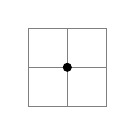
\begin{tikzpicture}
    \draw[step=0.5cm,gray,very thin] (0,0) grid (1,1);
    \draw[fill=black] (0.5,0.5) circle (0.05cm);
    \end{tikzpicture}
    \end{figure}

    The sample space is $\Omega = \{(x, y) \in \mathbb{R}^2: 0 \leq x \leq 1, 0 \leq y \leq 1\}$.


    
\end{frame}

\begin{frame}{Events}

\begin{itemize}
\item An event is a subset of the sample space.
\item For example, if we toss a coin, the sample space is  $\Omega = \{H, T\}$. The event that the coin lands heads is $A = \{H\}$.
\item If we toss two coins, the sample space is $\{HH, HT, TH, TT\}$. The event that the first coin lands heads is $A = \{HH, HT\}$.
\item If we toss a coin and roll a die, the sample space is $\{H1, H2, H3, H4, H5, H6, T1, T2, T3, T4, T5, T6\}$. The event that the coin lands heads is $A = \{H1, H2, H3, H4, H5, H6\}$.
\item If we measure the height of a person, the sample space is $\mathbb{R}$. The event that the height is greater than 6 feet is $A = \{x \in \mathbb{R}: x > 6\}$.
\end{itemize}
    
\end{frame}
\begin{frame}{Axioms of Probability}
    \begin{enumerate}
        \item $P(A) \geq 0$ for all events $A$.
        \item $P(\Omega) = 1$.
        \item If $A_1, A_2, \ldots$ are disjoint events, then $P(\cup_{i=1}^{\infty} A_i) = \sum_{i=1}^{\infty} P(A_i)$.
    \end{enumerate}
    
\end{frame}

\begin{frame}{Consequences of Axioms}
    \begin{enumerate}
        \item $P(\emptyset) = 0$.
        \item $P(A^c) = 1 - P(A)$.
        \item $P(A \cup B) = P(A) + P(B) - P(A \cap B)$.
        \item $P(A \cup B \cup C) = P(A) + P(B) + P(C) - P(A \cap B) - P(A \cap C) - P(B \cap C) + P(A \cap B \cap C)$.
    \end{enumerate}
\end{frame}
    
\begin{frame}{Conditional Probability}
    \begin{itemize}
        \item The conditional probability of $A$ given $B$ is defined as $P(A|B) = \frac{P(A \cap B)}{P(B)}$.
        \item If $A$ and $B$ are independent, then $P(A|B) = P(A)$.
        \item If $A$ and $B$ are independent, then $P(A \cap B) = P(A)P(B)$.
    \end{itemize}
    
\end{frame}

\begin{frame}{Random Variables}
    \begin{itemize}
        \item A random variable is a function from the sample space to the real numbers, i.e., $X: \Omega \rightarrow \mathbb{R}$.
        \item For example, if we toss a coin, the sample space is  $\Omega = \{H, T\}$. 
        \begin{itemize}
            \item We can define a random variable $X$ as $X(H) = 1$ and $X(T) = 0$.
            \item We could also have a random variable $Y$ to denote our gain from the coin toss, i.e., $Y(H) = 1$ and $Y(T) = -1$.
        \end{itemize}
        \item If we toss two coins, the sample space is $\{HH, HT, TH, TT\}$. 
        \begin{itemize}
            \item We can define a random variable $X$ as $X(HH) = 2$, $X(HT) = 1$, $X(TH) = 1$, and $X(TT) = 0$, where $X$ denotes the number of heads.
        \end{itemize}
    \end{itemize}

    %Add tcolorbox example to note the notation: X means random variable and x means a particular value of the random variable

    \begin{tcolorbox}[colback=metropolisblue!5,colframe=metropolisblue,title=Random Variables Notation]
        $X$ denotes a random variable. $x$ denotes a particular value of the random variable.
        %\item $P(X = x)$ denotes the probability that the random variable $X$ takes the value $x$.
    \end{tcolorbox}
    
\end{frame}

\begin{frame}{Probability Mass Function}
    \begin{itemize}
        \item The probability mass function (PMF) of a discrete random variable $X$ is defined as $p_X(x) = P(X = x)$.
        \item For example, if we toss a coin, the sample space is  $\Omega = \{H, T\}$. 
        \begin{itemize}
            \item We can define a random variable $X$ as $X(H) = 1$ and $X(T) = 0$.
            \item The PMF of $X$ is $p_X(1) = P(X = 1) = P(H) = 0.5$ and $p_X(0) = P(X = 0) = P(T) = 0.5$.
        \end{itemize}
        \item If we toss two coins, the sample space is $\{HH, HT, TH, TT\}$. 
        \begin{itemize}
            \item We can define a random variable $X$ as $X(HH) = 2$, $X(HT) = 1$, $X(TH) = 1$, and $X(TT) = 0$, where $X$ denotes the number of heads.
            \item The PMF of $X$ is $p_X(2) = P(X = 2) = P(HH) = 0.25$, $p_X(1) = P(X = 1) = P(HT) + P(TH) = 0.5$, and $p_X(0) = P(X = 0) = P(TT) = 0.25$.
        \end{itemize}
    \end{itemize}
    
\end{frame}

\begin{frame}{Probability Mass Function}
   Consider two rolls of die. The following is the sample space.

   \begin{table}[h]
    \centering
    \resizebox{0.3\textwidth}{!}{%
    \begin{tabular}{c|cccccc}
    \hline
    X/Y & 1 & 2 & 3 & 4 & 5 & 6 \\
    \hline
    1 & 11 & 12 & 13 & 14 & 15 & 16 \\
    2 & 21 & 22 & 23 & 24 & 25 & 26 \\
    3 & 31 & 32 & 33 & 34 & 35 & 36 \\
    4 & 41 & 42 & 43 & 44 & 45 & 46 \\
    5 & 51 & 52 & 53 & 54 & 55 & 56 \\
    6 & 61 & 62 & 63 & 64 & 65 & 66 \\
    \hline
    \end{tabular}%
    }
    \end{table}
    \begin{itemize}
        \item X and Y are random variables (value of the 1st and 2nd die)
        \item $p_X(1) = P(X = 1) = P(11) + P(11) + P(13) + P(14) + P(15) + P(16) = \frac{1}{6}$
    \end{itemize}

    % Draw the PMF of X using tikz or pgfplots as a simple bar plot. Each of the value X = 1, 2, .. has the same PMF of 1/6
    % Add the PMF of Y as well. Each of the value Y = 1, 2, .. has the same PMF of 1/6

    \begin{figure}
            
    
            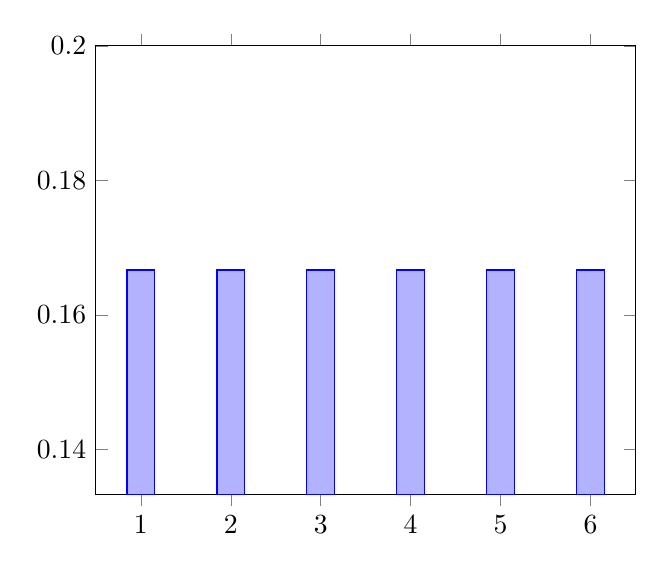
\begin{tikzpicture}
         
                \begin{axis} [ybar]
                \addplot coordinates {
                    (1,1/6) 
                    (2,1/6) 
                    (3,1/6) 
                    (4,1/6)
                    (5,1/6)
                    (6,1/6)
                };
                \end{axis}
                 
                \end{tikzpicture}
                \caption{PMF of X}
                \label{fig:my_label}
            \end{figure}

    
    
        





    
\end{frame}

\begin{frame}{Probability Mass Function}
    \begin{itemize}
        \item Let us create a new random variable Z = X + Y. 
        \begin{itemize}
            \item $p_Z(1) = 0$ as there is no way to get a sum of 1 from two die rolls.
            \item $p_Z(2) = P(Z = 2) = P(11) = \frac{1}{36}$
        \end{itemize}
    \end{itemize}
    
    \begin{figure}
        \centering
        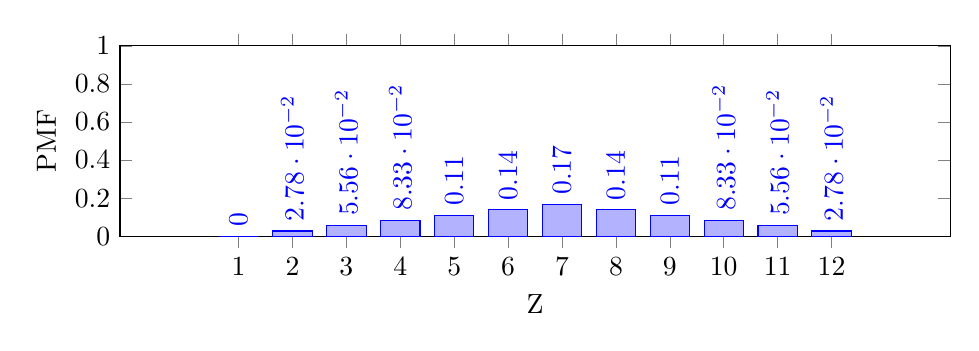
\begin{tikzpicture}
            \begin{axis} [
                ybar,
                ymin=0,
                ymax=1,
                xlabel={Z},
                ylabel={PMF},
                xtick=data,
                xticklabels={1, 2, 3, 4, 5, 6, 7, 8, 9, 10, 11, 12},
                width=\textwidth,
                height=4cm,
                bar width=0.5cm,
                enlarge x limits=0.2,
                nodes near coords,
                every node near coord/.append style={rotate=90, anchor=west},
            ]
            \addplot coordinates {
                (1, 0) 
                (2, 1/36) 
                (3, 2/36) 
                (4, 3/36)
                (5, 4/36)
                (6, 5/36)
                (7, 6/36)
                (8, 5/36)
                (9, 4/36)
                (10, 3/36)
                (11, 2/36)
                (12, 1/36)
            };
            \end{axis}
        \end{tikzpicture}
    \end{figure}
    
\end{frame}

\section{Discrete Random Variables}

\begin{frame}{Bernoulli Distribution}
    \begin{itemize}
        \item A random variable $X$ is said to follow a Bernoulli distribution with parameter $p$ if $X$ can take only two values, 0 and 1, and $P(X = 1) = p$.
        \item The PMF of $X$ is $p_X(x) = p^x(1 - p)^{1 - x}$.
        \item For example, if we toss a coin, the sample space is  $\Omega = \{H, T\}$. 
        \begin{itemize}
            \item We can define a random variable $X$ as $X(H) = 1$ and $X(T) = 0$.
            \item The PMF of $X$ is $p_X(1) = P(X = 1) = P(H) = p$ and $p_X(0) = P(X = 0) = P(T) = 1 - p$.
        \end{itemize}
    \end{itemize}

    \begin{figure}
        
 
        \pgfmathsetmacro{\p}{0.7}
        \pgfmathsetmacro{\q}{1-\p}
        
        \begin{tikzpicture}
          \begin{axis}[
            ybar,
            ymin=0,
            ymax=1,
            xlabel={X},
            ylabel={PMF},
            xtick={0,1},
            xticklabels={0,1},
            width=5cm,
            height=3cm,
            bar width=0.8cm,
            enlarge x limits=0.5,
          ]
          \addplot coordinates {(0, \q) (1, \p)};
          \end{axis}
        \end{tikzpicture}
        
         \end{figure}
      
    
\end{frame}


\end{document}







\end{document}